\section{Structure de la peau}
\label{sec:orgcf08ddd}
\begin{figure}[htbp]
\centering
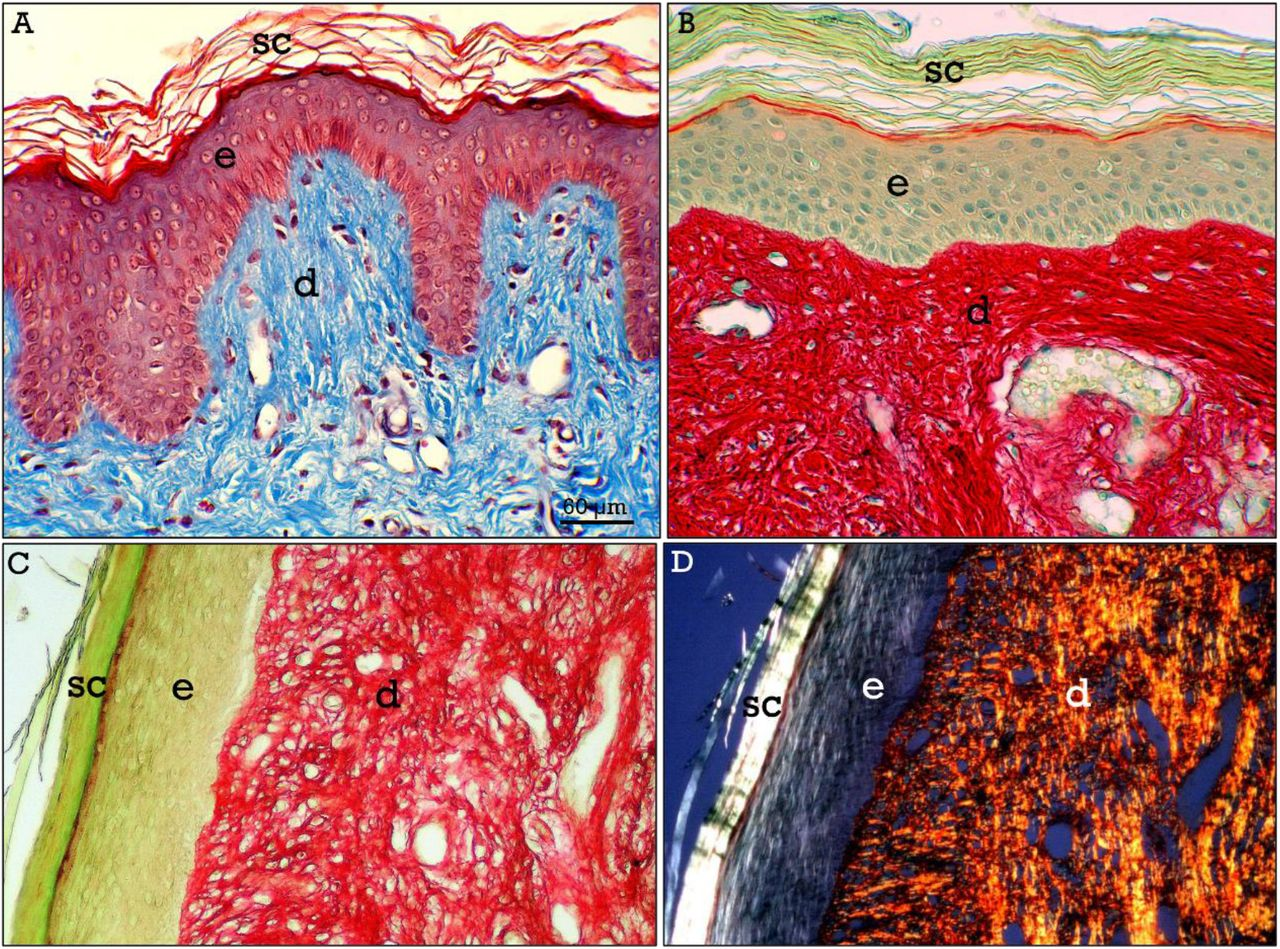
\includegraphics[width=.9\linewidth]{/img/skin/F15.large.jpg}
\caption{\emph{\protect\hyperlink{gls-1}{\label{gls-1-use-1}Trichrome de Masson}} sur biopsies de la peau #cite(label("serrano-garridoStainingHumanSkin2022"))}
\end{figure}
\subsection{Anatomie}
\label{sec:org12c7c34}
La peau est composée de trois couches principales: 

\begin{itemize}
\item \textbf{L'épiderme}: Correspond à la couche externe de la peau. Constituée de
\protect\hyperlink{gls-2}{\label{gls-2-use-1}kératinocytes}, elle a un rôle important dans la protection du corps contre
différents élements\footnote{Bactéries, UV#cite(label("brennerProtectiveRoleMelanin2008")), irritants}
\begin{quote}
L’épiderme est un épithélium de revêtement, stratifié, pavimenteux, orthokératosique, non vascularisé mais innervé.
\end{quote}

\item \textbf{Le derme}: Très vascularisé\footnote{Contrairement à l'épiderme}, permet l'irrigation et la régulation de l'épiderme.

\item \textbf{L'hypoderme} (ou tissu sous-cutané): C'est la couche la plus profonde de la peau, composée principalement de tissu adipeux. Elle sert de réserve énergétique, d'isolant thermique et de coussin protecteur pour les organes internes contre les chocs extérieurs.
\end{itemize}
\subsection{Fonctions de la peau}
\label{sec:orgff89a5f}
La peau remplit diverses fonctions vitales :

\begin{itemize}
\item \textbf{Protection} :
\item Régulation thermique : Grâce à la sudation et à la vasodilatation, elle participe à la régulation de la température corporelle.
\item \textbf{Sensation} : Les nombreuses terminaisons nerveuses présentes dans le derme permettent de percevoir la douleur, le toucher, la chaleur et le froid.
\item \textbf{Synthèse de la vitamine D} : Sous l'effet des rayons UVB, la peau joue un rôle
crucial dans la synthèse de la vitamine D, indispensable à l'homéostasie
calcique.
\end{itemize}
\section{Index}
\label{sec:org4021963}
\hypertarget{gls-1}{Kératinocytes}\hspace*{.5em}\pageref{gls-2-use-1}

\hypertarget{gls-2}{Trichrome de Masson}\hspace*{.5em}\pageref{gls-1-use-1}
